
% JuliaCon proceedings template
\documentclass{juliacon}

% math
\usepackage{amsmath}

% algorithm floats + pseudocode
\usepackage{algorithm}
\usepackage{algpseudocode}

% subfigures
\let\subcaption\relax
\let\subfloat\relax
\usepackage{subcaption}

% refs
\usepackage{cleveref}
\usepackage{placeins}

\usepackage{listings}
\lstset{
  breaklines=true,
  breakatwhitespace=true,
  columns=fullflexible
}

% Define the \add command
 \newcommand{\add}[1]{\textit{\textcolor{blue}{#1}}}
\newcommand{\dms}[1]{{\color{blue} \sf DMS: [#1]}}

% FIX COLOR LEAKING IN .STY (THAT WE SHOULDN'T TOUCH)
\makeatletter
\renewcommand{\lstbasicfont}{%
  \ttfamily
  \lst@ifdisplaystyle\scriptsize\fi
}
\makeatother

\color{black}
% END OF THE FIX

\setcounter{page}{1}

\begin{document}

% **************GENERATED FILE, DO NOT EDIT**************

\title{GraphLab.jl: A Julia Framework for Graph Partitioning}

\author[1]{Malik Lechekhab}
\author[1]{Dimosthenis Pasadakis}
\author[2]{Roger K{\"a}ppeli}
\author[1]{Aryan Eftekhari}
\author[1]{Olaf Schenk}
\affil[1]{Faculty of Informatics, Universit{\`a} della Svizzera italiana}
\affil[2]{Seminar for Applied Mathematics, ETH Z{\"u}rich}

\keywords{Julia, Graph algorithms, Graph partitioning, Recursive methods, Numerical computing}

\hypersetup{
pdftitle = {GraphLab.jl: A Julia Framework for Graph Partitioning},
pdfsubject = {JuliaCon 2019 Proceedings},
pdfauthor = {Malik Lechekhab, Dimosthenis Pasadakis, Roger K{\"a}ppeli, Aryan Eftekhari, Olaf Schenk},
pdfkeywords = {Julia, Graph algorithms, Graph partitioning, Recursive methods, Numerical computing},
}



\maketitle

\begin{abstract}
    %%%%%%%%%%%%%%%%%%%%%%%%%%%%%%%%%%%%%%%%%%%%%%%%%%%%%%%%%%%%%%
% Abstract
%%%%%%%%%%%%%%%%%%%%%%%%%%%%%%%%%%%%%%%%%%%%%%%%%%%%%%%%%%%%%%
    We design and implement \texttt{GraphLab.jl}, a \texttt{Julia} package facilitating the study, experimentation, and research of
    graph partitioning. \texttt{GraphLab.jl} explores the principles and trade-offs of partitioning
    algorithms. It offers a set
    of methods, including coordinate, inertial, and spectral
    bisection, random spheres, space-filling curves, and nested
    dissection, with support for recursive partitioning.
    The
    package includes routines for generating adjacency matrices, 
    computing partition quality metrics, benchmarking problems,
    and visualizing partitioned graphs. 
    % Our work provides a \texttt{Julia}-based framework to learners and researchers engaging in
    % graph theory and related partitioning problems. 
    % \textcolor{red}{AE NOTE :  What do you mean "growing set" ? How is it growing? we are just introducing it. I would remove this.}

    % \textcolor{red}{AE NOTE: "routines for benchmarking problems" or routines for "benchmark problems"?}
    % \texttt{GraphLab.jl}
    % enables integration with external graph partitioning software, thus allowing users to compare additional methods and results in a unified environment. 
    % \textcolor{red}{AE NOTE: You are starting the sentence two times with "GraphLab.jl". }
    % \textcolor{red}{AE NOTE:  Don't start with "last" if you have not stated "first" or "second"  above, maybe you mean "finally"?  This sentence is somewhat redundant and overlaps with the first sentence of the abstract, which already states that it "facilitates the study, experimentation, and research of graph partitioning". }



% Old abstract

    % \texttt{GraphLab.jl} is a Julia package designed to facilitate the study, experimentation, and research of graph partitioning. \texttt{GraphLab.jl} provides a framework for exploring the principles and trade-offs of partitioning algorithms through hands-on tools. It implements a growing set of methods—including coordinate, inertial, and spectral bisection, random spheres, space-filling curves, and nested dissection—with support for recursive partitioning. The package includes routines for generating adjacency matrices, computing partition quality metrics, benchmarking problems, and visualizing partitioned graphs. \texttt{GraphLab.jl} enables integration with external graph partitioning software, thus allowing users to compare additional methods and results in a unified environment. This work also aims to introduce Julia's capabilities to learners and researchers engaging in graph theory and related partitioning problems.



% Vey Old abstract

    % Partitioning computational problems into smaller problems that can be
    % efficiently solved in parallel is fundamental in high-performance computing
    % (HPC). Effective partitioning requires balancing subproblem sizes to
    % ensure load distribution while minimizing inter-problem communication.
    % We develop a comprehensive framework that streamlines the study and exploration of graph partitioning. It provides implementations of fundamental partitioning algorithms, visualization tools, adjacency matrix construction utilities, partition quality metrics, and benchmarking capabilities.
    % Additionally, the framework integrates with popular graph partitioning
    % software, facilitating systematic investigation, experimentation and visualization in graph partitioning.
\end{abstract}

\section{Introduction}
    %%%%%%%%%%%%%%%%%%%%%%%%%%%%%%%%%%%%%%%%%%%%%%%%%%%%%%%%%%%%%%
% Introduction
%%%%%%%%%%%%%%%%%%%%%%%%%%%%%%%%%%%%%%%%%%%%%%%%%%%%%%%%%%%%%%
\documentclass[../paper.tex]{subfiles}
\begin{document}

% \textcolor{red}{AE NOTE: here you should outline different package that exist that do the same things ( be it for different programming languages).}

    Graph partitioning is a fundamental problem with wide-ranging
    applications in computational
    biology, high-performance
    computing, and distributed
    systems, among many other
    domains~\cite{buluc2015recentadvancesgraphpartitioning}. Partitioning large graphs into loosely connected
    subsets of roughly equal size promotes parallel execution,
    reduces communication overhead, and provides insights into the
    structure of complex networks~\cite{MoreRecentAdvances}.

    %  
    We contribute to the \texttt{Julia} ecosystem of graph algorithms with
    \texttt{GraphLab.jl}, a package designed to
    facilitate the study, experimentation, and research
    of graph partitioning.
    Similar to existing toolboxes such as \texttt{meshpart}~\cite{gilbert_2020_3746723} in \texttt{MATLAB}, and \texttt{CDLIB}~\cite{Rossetti2019} in \texttt{Python}, which focuses on community detection, \texttt{GraphLab.jl} aims to offer a framework for graph partitioning in \texttt{Julia}.
    A diverse set of partitioning algorithms are implemented in
    the introduced package, including
    coordinate~\cite{Simon91}, inertial~\cite{farhat1993automatic}, and
    spectral bisection~\cite{fiedler75,Simon91}, random spheres~\cite{doi:10.1137/S1064827594275339}, space-filling
    curves~\cite{Sasidharan15}, and nested dissection~\cite{George73}. These methods can be applied
    recursively for hierarchical partitioning or fill-in reducing strategies. \texttt{GraphLab.jl} also
    provides routines for generating adjacency matrices based on coordinate systems, computing partition quality metrics,
    benchmarking problems, and visualizing partitioned graphs.
    
    The paper is structured as follows. \Cref{sec:background}
    provides a brief background on
    graph partitioning, followed by an
    overview of the fundamental implemented partitioning
    algorithms in \Cref{sec:algo}. \Cref{sec:framwork} introduces
    our framework, detailing its capabilities in graph creation,
    partitioning, benchmarking and visualization. Installation
    and usage
    demonstrations are presented in \Cref{sec:demo}, and we
    conclude with a summary and directions for future work in
    \Cref{sec:conclusion}.
\end{document}
    % \textcolor{red}{AE NOTE: of the}

    
    % Over the years, a plethora of graph partitioning
    % techniques has been developed~\cite{MoreRecentAdvances, DBLP:conf/wea/SandersS13}. 
    % \texttt{GraphLab.jl} enables users to experiment with algorithms, compare methods, and visualize results, thereby serving as a learning and research tool for graph partitioning.

    
    % (\textcolor{red}{AE NOTE: i think this should be "has".})
    % \textcolor{red}{AE NOTE: I think this is a bit imprecise ... if we want to say " it serves as learning tool because it lets one compare methods easily" that we should say that directly. }
    % \texttt{GraphLab.jl} offers a framework
    % that enables users to experiment with algorithms, 
    % visualize results, and assess partition quality.


    % It allows integration with external
    % graph partitioning software, thus allowing users to compare additional methods and results in a
    % unified environment.

    % This work aims to contribute to the educational efforts of the Julia graph community and to assist in introducing Julia's capabilities to learners and researchers engaging in graph theory and related partitioning problems.
    





    % Graph partitioning is a fundamental problem with broad applications in scientific domains where the relationships between interconnected variables are critical. From computational biology and social network analysis to high-performance computing (HPC) and distributed systems, efficient graph partitioning techniques play a key role in optimizing performance, reducing computational overhead, and enabling deeper insight into complex data.



    % Over the years, a diverse array of graph partitioning techniques has been developed, including spectral partitioning, multilevel approaches, and combinatorial optimization methods. While these techniques have significantly advanced the field, teaching and experimenting with them --- particularly in an HPC context --- pose unique challenges. For both students and researchers, the ability to explore multiple partitioning strategies, evaluate their effectiveness, and compare their trade-offs is essential to develop an intuitive understanding of graph partitioning.
    
    % To facilitate this process, we introduce a framework, \texttt{\texttt{GraphLab.jl}}, designed to support the study and benchmarking of graph partitioning techniques within a unified workflow. Implemented in Julia, \texttt{\texttt{GraphLab.jl}} does not aim to replace existing graph processing and visualization tools, but rather to integrate them, offering a cohesive environment where users can construct graphs, apply partitioning algorithms, analyze and visualize the results seamlessly. It supports both recursive and non-recursive partitioning strategies, including geometric approaches such as coordinate bisection and inertial bisection, as well as methods that operate without geometric data, such as spectral bisection. The framework provides tools for visualization, quality assessment, and performance benchmarking, offering a structured workflow for both research and education.
    
    % We selected Julia as the foundation for this framework due to its modern, high-performance architecture, user-friendly syntax, and strong commitment to open-source principles. Julia’s accessibility and reproducibility make it particularly well suited for interactive exploration and algorithmic experimentation. To further enhance usability, the framework integrates seamlessly with \texttt{Pluto.jl} notebooks, creating an interactive environment for hands-on learning and pedagogical applications.
    
    % Although our framework provides essential partitioning tools, it also allows users to incorporate external graph partitioning software, facilitating interoperability with established libraries and algorithms. We offer guidelines and examples for integrating widely used partitioning tools into Julia workflows, allowing researchers to take advantage of the latest methods alongside the capabilities of our framework.

\section{Background on graph partitioning}
    \label{sec:background}
    %%%%%%%%%%%%%%%%%%%%%%%%%%%%%%%%%%%%%%%%%%%%%%%%%%%%%%%%%%%%%%
% Background
%%%%%%%%%%%%%%%%%%%%%%%%%%%%%%%%%%%%%%%%%%%%%%%%%%%%%%%%%%%%%%
\documentclass[../paper.tex]{subfiles}
\begin{document}
    Consider a mesh consisting of eight cells, as illustrated in \Cref{fig:mesh_example}.
    If data exchange occurs only between adjacent cells, the mesh can be represented as a dependency
    graph, shown in \Cref{fig:graph_example}.
    To partition the mesh into two domains suitable for parallel processing, the objective
    is to divide it into two submeshes of equal size while
    minimizing the number of edges connecting them.
    This corresponds to partitioning the original graph into two complementary 
    subgraphs of equal number of vertices and with a minimum number of interconnecting edges.
    % In other words, the graph is divided into two balanced subsets by cutting the minimal
    % number of edges.
    
    \begin{figure}[h!]
        \centering
        \begin{subfigure}[b]{0.23\textwidth}
            \centering
            \includegraphics[width=\textwidth]{images/mesh.drawio.svg.pdf}
            \caption{}
            \label{fig:mesh_example}
        \end{subfigure}
        \hfill
        \begin{subfigure}[b]{0.23\textwidth}
            \centering
            \includegraphics[width=\textwidth]{images/graph.drawio.svg.pdf}
            \caption{}
            \label{fig:graph_example}
        \end{subfigure}
        \caption{Mesh example consisting of 8 parts (left) and the corresponding
        dependency graph (right).}
        \label{fig:mesh_and_graph}
    \end{figure}
    
    
    However, for this bisection problem, finding an optimal solution is NP-hard, making exact computation intractable for large instances \cite{buluc2015recentadvancesgraphpartitioning}. In the following,
    we formalize the graph partitioning problem and introduce bisection algorithms.
    Here, \textit{bisection} specifically refers partitioning the graph into two sub-graphs.
    A general partitioning into $p = 2^l$ sub-graphs can then
    be obtained recursively by applying these bisection methods iteratively.
    
    Let $G=(\mathcal{V}, \mathcal{E})$ be an undirected graph with a vertex set 
    $\mathcal{V}=\{ v_1, \dots, v_n \}$ where each vertex $v_i$ represents
    an element or entity in the problem domain, and an edge set $\mathcal{E}$
    where each edge $e_{i, j} \in \mathcal{E}$ represents a symmetric relation between
    two distinct vertices $v_i$ and $v_j$, meaning that
    $e_{i, j} \in \mathcal{E}$ implies $e_{j, i} \in \mathcal{E}$, and no self-loops exist, i.e., $e_{i, i} \notin \mathcal{E}$. Graphs satisfying these properties are formally referred to as simple and undirected.
    
    The adjacency matrix $\mathbf{A} \in \mathbb{R}^{n \times n}$ of the graph
    stores the connectivity information among its vertices, where the entry
    $\mathbf{A}_{ij}$ is defined as:
    \begin{equation}
      \mathbf{A}_{ij} =
        \begin{cases}
            a_{ij}, & \text{if } e_{i,j} \in \mathcal{E},\\
            0, & \text{otherwise}.
        \end{cases}
    \end{equation}
    
    Here, $a_{ij}$ represents the weight of the edge $e_{i,j}$, which is a nonnegative real-valued number indicating the strength or capacity of the connection
    between vertices $v_i$ and $v_j$. In unweighted graphs, $a_{ij}$ simplifies to 1 for all connected pairs.
    For the simple undirected graphs considered here,the adjacency matrix is symmetric, satisfying $a_{ij} = a_{ji}$ with a zero diagonal, i.e., $a_{ii} = 0$.
    The degree of a vertex $v_i$, denoted as $d_i = \sum^n_j a_{ij}$, represents the sum of the weights of edges incident to $v_i$. In unweighted graphs, $d_i$ reduces to the number of edges connecting $v_i$, effectively counting its direct
    neighbors. The degree matrix $\mathbf{D} \in \mathbb{R}^{n \times n}$ is defined
    as a diagonal matrix, where the diagonal entries correspond to the degrees of all vertices $d_1, \dots, d_n$.
    
    As an example, for the mesh and the corresponding graph depicted in \Cref{fig:mesh_and_graph}, the adjacency matrix $\mathbf{A}$ and the degree matrix $\mathbf{D}$ are given as follows:
    
    \vspace{5mm}
    
    $ \mathbf{A}=
    \begin{pmatrix}
    \color{lightgray} 0 & 1 & \color{lightgray} 0 & \color{lightgray} 0 & \color{lightgray} 0 & 1 & \color{lightgray} 0 & \color{lightgray} 0 \\
    1 & \color{lightgray} 0 & 1 & \color{lightgray} 0 & \color{lightgray} 0 & \color{lightgray} 0 & \color{lightgray} 0 & \color{lightgray} 0 \\
    \color{lightgray} 0 & 1 & \color{lightgray} 0 & 1 & \color{lightgray} 0 & \color{lightgray} 0 & \color{lightgray} 0 & \color{lightgray} 0 \\
    \color{lightgray} 0 & \color{lightgray} 0 & 1 & \color{lightgray} 0 & 1 & \color{lightgray} 0 & \color{lightgray} 0 & \color{lightgray} 0 \\
    \color{lightgray} 0 & \color{lightgray} 0 & \color{lightgray} 0 & 1 & \color{lightgray} 0 & 1 & \color{lightgray} 0 & \color{lightgray} 0 \\
    1 & \color{lightgray} 0 & \color{lightgray} 0 & \color{lightgray} 0 & 1 & \color{lightgray} 0 & 1 & \color{lightgray} 0 \\
    \color{lightgray} 0 & \color{lightgray} 0 & \color{lightgray} 0 & \color{lightgray} 0 & \color{lightgray} 0 & 1 & \color{lightgray} 0 & 1 \\
    \color{lightgray} 0 & \color{lightgray} 0 & \color{lightgray} 0 & \color{lightgray} 0 & \color{lightgray} 0 & \color{lightgray} 0 & 1 & \color{lightgray} 0 
    \end{pmatrix},
    \mathbf{D}=
    \begin{pmatrix}
    2 & \color{lightgray} 0 & \color{lightgray} 0 & \color{lightgray} 0 & \color{lightgray} 0 & \color{lightgray} 0 & \color{lightgray} 0 & \color{lightgray} 0 \\
    \color{lightgray} 0 & 2 & \color{lightgray} 0 & \color{lightgray} 0 & \color{lightgray} 0 & \color{lightgray} 0 & \color{lightgray} 0 & \color{lightgray} 0 \\
    \color{lightgray} 0 & \color{lightgray} 0 & 2 & \color{lightgray} 0 & \color{lightgray} 0 & \color{lightgray} 0 & \color{lightgray} 0 & \color{lightgray} 0 \\
    \color{lightgray} 0 & \color{lightgray} 0 & \color{lightgray} 0 & 2 & \color{lightgray} 0 & \color{lightgray} 0 & \color{lightgray} 0 & \color{lightgray} 0 \\
    \color{lightgray} 0 & \color{lightgray} 0 & \color{lightgray} 0 & \color{lightgray} 0 & 2 & \color{lightgray} 0 & \color{lightgray} 0 & \color{lightgray} 0 \\
    \color{lightgray} 0 & \color{lightgray} 0 & \color{lightgray} 0 & \color{lightgray} 0 & \color{lightgray} 0 & 3 & \color{lightgray} 0 & \color{lightgray} 0 \\
    \color{lightgray} 0 & \color{lightgray} 0 & \color{lightgray} 0 & \color{lightgray} 0 & \color{lightgray} 0 & \color{lightgray} 0 & 2 & \color{lightgray} 0 \\
    \color{lightgray} 0 & \color{lightgray} 0 & \color{lightgray} 0 & \color{lightgray} 0 & \color{lightgray} 0 & \color{lightgray} 0 & \color{lightgray} 0 & 1 
    \end{pmatrix}
    $
    
    \vspace{5mm}
    
    We refer the reader to \cite{doi:https://doi.org/10.1002/9781118601181.ch1} for a detailed overview of commonly used matrices and objectives functions in graph partitioning.
\end{document}

\section{Overview of implemented partitioning algorithms}
    \label{sec:algo}
    %%%%%%%%%%%%%%%%%%%%%%%%%%%%%%%%%%%%%%%%%%%%%%%%%%%%%%%%%%%%%%
% Algorithms
%%%%%%%%%%%%%%%%%%%%%%%%%%%%%%%%%%%%%%%%%%%%%%%%%%%%%%%%%%%%%%
% \documentclass[../paper.tex]{subfiles}
% \begin{document}
    This section provides an overview of the partitioning algorithms implemented
    in the framework, detailing their underlying principles.
    Through illustrative examples and visual representations, we highlight the behavior of each algorithm.

%%%%%%%%%%%%%%%%%%%%%%%%%%%%%%%%%%%%%%%%%%%%%%%%%%%%%%%%%%%%%%
% Geometric-based
%%%%%%%%%%%%%%%%%%%%%%%%%%%%%%%%%%%%%%%%%%%%%%%%%%%%%%%%%%%%%%
    \subsection{Geometric-based partitioning algorithms}
    \label{subsec:geo}
    This class of bisection algorithms operates under the assumption that the geometric layout of the
    graph is known.
    These algorithms exploit spatial information of the vertices to guide the
    partitioning process, aiming to minimize edge cuts while preserving geometric
    coherence~\cite{doi:10.1137/S1064827594275339}.
    This approach is particularly well suited for applications where the graph structure
    arises from physical systems, such as finite element meshes in numerical computing,
    where the underlying geometry directly influences computational efficiency~\cite{buluc2015recentadvancesgraphpartitioning}. Unless stated otherwise, all function calls presented in this section take as input a graph adjacency matrix \texttt{A} and a node coordinate matrix \texttt{coords}, and return a vector assigning each node to partition 1 or 2.
%%%%%%%%%%%%%%%%%%%%%%%%%%%%%%%%%%%%%%%%%%%%%%%%%%%%%%%%%%%%%%    
    \subsubsection{Coordinate bisection}
    \label{subsubsec:coord}
    Coordinate bisection seeks a hyperplane orthogonal to one of the coordinate axes that partitions the graph's vertices into two subsets of approximately equal size
    while minimizing the edge cut.
    The algorithm computes the median $\bar{x}_j$ of each coordinate $x_j$,
    dividing all graph vertices into two groups: one containing vertices with $x_j \leq \bar{x}_j$ and the other $x_j > \bar{x}_j$. The edge cut is then evaluated for each coordinate axis, and the
    partitioning is performed along the axis that yields the smallest edge cut.
    This process in a $d$-dimensional space is summarized in \Cref{alg:coord}, with a two-dimensional example illustrated in \Cref{fig:coord}.
    The complexity of coordinate bisection is $O(d(n+m))$ when using linear-time median selection or $O(d(n \log n + m))$ with sorting-based medians~\cite{10.5555/1614191}, where $n$ is the number of vertices, and $m$ the number of edges.

    
    \begin{figure}[h!]
    \centering
    \begin{subfigure}[b]{0.23\textwidth}
        \centering
        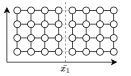
\includegraphics[width=\textwidth]{images/coord_1.drawio.svg.pdf}
        \caption{}
        \label{fig:coord_1}
    \end{subfigure}
    \hfill
    \begin{subfigure}[b]{0.23\textwidth}
        \centering
        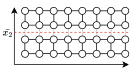
\includegraphics[width=\textwidth]{images/coord_2.drawio.svg.pdf}
        \caption{}
        \label{fig:coord_2}
    \end{subfigure}
    \caption{Bisection of the graph along the $x_1$-axis, resulting in a 4-edge cut (left),
    and along the $x_2$-axis, resulting in 8-edge cut (right). The $x_1$-axis bisection is selected.}
    \label{fig:coord}
\end{figure}
    \begin{algorithm}
    \caption{Coordinate bisection.}
    \label{alg:coord}
    \begin{algorithmic}[1]
        \Require Graph \( G = (\mathcal{V}, \mathcal{E}) \), points \( P_i = (x_{1}, \dots, x_{d})_i \)
        \Ensure A bisection of \( G \) into \(\mathcal{V}_1\) and \(\mathcal{V}_2\)
        \Function{coordinate\_part}{graph $G$, points $P_i$}
            \State Initialize $c_{\min} \gets \infty$, $j^* \gets 1$
            \For{each axis \( x_j \), \( j = 1, \dots, d \)}
                \State Compute the median \(\bar{x}_j\)
                \State Compute the edge cut \( c_j \) for the bisection at \(\bar{x}_j\)
                \If{ \( c_j < c_{\min} \) }
                    \State $c_{\min} \gets c_j$
                    \State $j^* \gets j$
                \EndIf
            \EndFor
            \State Partition \(\mathcal{V}\) into \(\mathcal{V}_1\) and \(\mathcal{V}_2\) via \(\bar{x}_{j^*}\) bisection
            \State \Return \(\mathcal{V}_1, \mathcal{V}_2\)
        \EndFunction
    \end{algorithmic}
\end{algorithm}
    
    The coordinate bisection method in \texttt{GraphLab.jl} can be invoked using the following command:
    
    \begin{lstlisting}[language=Julia]
    GraphLab.part_coordinate(A, coords)
    \end{lstlisting}
    
    The coordinate bisection algorithm is computationally efficient and conceptually simple.
    However, its effectiveness is strongly influenced by the choice of coordinate system.
    A mere rotation of the coordinate axes can lead to significantly different partitioning results,
    as the algorithm strictly aligns the division with the coordinate axes.
    This sensitivity may lead to suboptimal partitions, particularly in cases where the problem geometry
    is not naturally aligned with the axes.
%%%%%%%%%%%%%%%%%%%%%%%%%%%%%%%%%%%%%%%%%%%%%%%%%%%%%%%%%%%%%%   
    \subsubsection{Inertial bisection}
    The inertial bisection mitigates the axis-alignment limitation of coordinate bisection by
    allowing the dividing hyperplane to be orthogonal to a direction determined by the
    distribution of vertices rather than a fixed coordinate axis. Physically, this direction corresponds to the axis of minimal rotational inertia~\cite{elsner1997graph}, ensuring that
    partitioning is guided by the intrinsic geometry of the data rather than an arbitrary reference frame.
    
    In two dimensions, the dividing hyperplane is
    represented by a line $l$ that minimizes the sum
    of squared distances from the vertices to the line. The algorithm first determines the center of mass of the vertex set,
    \begin{equation}
      \bar{P}=(\bar{x}, \bar{y}), \quad \text{where} \quad  \bar{x} = \frac{1}{n}\sum_{i=1}^n x_i, \quad \bar{y} = \frac{1}{n}\sum_{i=1}^n y_i\text{.}
    \end{equation}
    It then defines a unit direction vector $\mathbf{u}=[u_1, u_2]^T$, such that 
    $\|\mathbf{u}\|_2 = \sqrt{u_1^2+u_2^2} = 1$.
    The parametric equation
    of the bisecting line is given by
    $l(\lambda) = \{\bar{P} + \lambda \mathbf{u}  \mid \lambda \in \mathbb{R} \}$.
    
    \begin{figure}[h!]
    \centering
    \begin{subfigure}[b]{0.23\textwidth}
        \centering
        \includegraphics[width=\textwidth]{images/inert_0.drawio.svg.pdf}
        % \caption{}
        \label{fig:inert_1}
    \end{subfigure}
    \hfill
    \begin{subfigure}[b]{0.23\textwidth}
        \centering
        \includegraphics[width=\textwidth]{images/inert.drawio.svg.pdf}
        % \caption{}
        \label{fig:inert_2}
    \end{subfigure}
    \caption{Illustration of the inertial bisection in 2D: dividing the graph
    along the line orthogonal to the direction $\mathbf{u}$ through the center of mass $\bar{P}$ that minimizes the sum of squared distances.}
    \label{fig:inert}
\end{figure}
    
    % The coordinates of the center of mass $\bar{P}$, which lies on the line $l$, are given by
    
    
    To determine the optimal orientation of the bisecting hyperplane, the unit direction vector $\mathbf{u}$ is chosen to minimize the sum of the squared
    distances from the vertices to the line. In the case of a two-dimensional graph embedding, this reads:
    
    \begin{equation} 
\begin{aligned}[b]
    \sum_{i=1}^n d_i^2 
    &= \sum_{i=1}^n(x_i - \bar{x})^2+(y_i - \bar{y})^2\\
    &-(u_1(x_i - \bar{x})+u_2(y_i - \bar{y}))^2 \\
    &=(1-u_1^2)\sum_{i=1}^n(x_i - \bar{x})^2+
    (1-u_2^2)\sum_{i=1}^n(y_i - \bar{y})^2\\
    &+2u_1u_2\sum_{i=1}^n(x_i - \bar{x})(y_i - \bar{y})\\
    &= (1-u_1^2)S_{xx}+
    (1-u_2^2)S_{yy}+2u_1u_2S_{xy}\\
    &=\mathbf{u}^T
    \vcenter{
        \hbox{$
        \begin{pmatrix}
        S_{xx} & S_{xy} \\
        S_{xy} & S_{yy}
        \end{pmatrix}
        $}
    } \label{eq:projection_matrix}
    \mathbf{u} = \mathbf{u}^T\mathbf{M}\mathbf{u}
\end{aligned}
\end{equation}
    
    Here, $\mathbf{M}$ is a symmetric matrix, and its smallest eigenvalue corresponds to the minimal sum of the squared distances. Consequently, the optimal direction vector $\mathbf{u}$ is given by the
    normalized eigenvector associated with the smallest eigenvalue of
    $\mathbf{M}$~\cite{elsner1997graph}. This choice ensures that the partitioning hyperplane is aligned with the principal axis of least variance, making the algorithm robust to coordinate system transformations. The full procedure for bisecting a graph using inertial partitioning is summarized in \Cref{alg:inert}.
    The inertial bisection runs in time $O(nd+m+d^3)$, which simplifies to $O(n+m)$ in fixed spatial dimension.
    
    \begin{algorithm}
    \caption{Inertial bisection.}
    \label{alg:inert}
    \begin{algorithmic}[1]
        \Require Graph \( G = (\mathcal{V}, \mathcal{E}) \), points \( P_i = (x_{1}, \dots, x_{d})_i \)
    \Ensure A bisection of \( G \) into \(\mathcal{V}_1\) and \(\mathcal{V}_2\)
    \Function{inertial\_part}{graph $G$, points $P_i$}
        \State Calculate the center of mass $\bar{P}$
        \State Compute eigenvec. associated with smallest eigenval. of $\mathbf{M}$
        \State Partition the vertices $\mathcal{V}$ around the line $l$
        \State \Return \(\mathcal{V}_1, \mathcal{V}_2\)
    \EndFunction
    \end{algorithmic}
\end{algorithm}

    To perform inertial bisection with \texttt{GraphLab.jl} on a graph, use:

    \begin{lstlisting}[language=Julia]
    GraphLab.part_inertial(A, coords)
    \end{lstlisting}

%%%%%%%%%%%%%%%%%%%%%%%%%%%%%%%%%%%%%%%%%%%%%%%%%%%%%%%%%%%%%%
    \subsubsection{Random sphere bisection}
    \label{sub:rand_sphere}

    The random sphere method~\cite{doi:10.1137/S1064827594275339} partitions a graph
    by exploiting spatial information to identify separators aligned with the intrinsic geometry of the vertex
    distribution.
    Unlike axis-aligned or inertia-based approaches,
    it employs randomized geometric projections to discover low-cut partitions.
    
    Given vertex coordinates $P_i = (x_1, \dots, x_d)_i$, the algorithm first computes the center of mass $\bar{P}$ and normalizes the coordinates as
    \begin{equation}
        \tilde{P}_i=\frac{P_i-\bar{P}}{\max_j{|P_j-\bar{P}|}},
    \end{equation}
    so that the distribution is centered at the origin and confined within a unit-scale region.
    Each normalized point $\tilde{P}_i$ is then mapped to the unit sphere,
    $Z_i \in \mathcal{S}^d \subset{\mathbb{R}^{d+1}}$, via stereographic projection.

    To identify separators, the algorithm selects $s$ random center points on the sphere.
    Each center $c$ is computed as the coordinate-wise median of a randomly sampled subset of vertices and then moved to the origin through a conformal transformation of the sphere.
    For each transformed configuration, several random unit directions $u$ are sampled, and a candidate spherical cut is generated as

    \begin{equation}
        \mathcal{V}_1= \{ i \mid \langle Z_i, u \rangle \leq 0 \}, \quad \mathcal{V}_2 = \{ i \mid \langle Z_i, u \rangle > 0 \},
    \end{equation}
    The corresponding edge cut is evaluated, and the partition with the smallest cut is retained.

    % 
    \begin{figure}[t]
    \centering
    \includegraphics[width=1.0\linewidth]{images/rsphere.png}
    \caption{
    % Spectral embedding and random sphere partitioning: the graph is first embedded into a 2-dimensional
    % spectral space using the eigenvectors associated with the second and third smallest eigenvalues of the graph Laplacian. A separator (shown in red)
    % is then selected using the randomized sphere method and mapped back onto original graph.
    Random sphere partitioning: the 2D coordinates of \texttt{mesh1e1}~\cite{10.1145/2049662.2049663} are normalized and stereographically lifted to the sphere $\mathcal{S}^2 \subset \mathbb{R}^3$, where a centerpoint $c$ is computed and mapped to the origin via a conformal transformation. A direction $\mathbf{u}$ defining a circle separator (shown in red) is then selected, partitioning the spherical embedding. The resulting partition is projected onto the original layout. 
    }
    \label{fig:rsphere}
    \end{figure}
    % 

    In addition to spherical separators, the algorithm also considers random linear cuts in the original
    Euclidean space, defined by hyperplanes
    orthogonal to random directions and positioned at the median projected vertex coordinates.
    The final output is the spherical or linear bisection minimizing the total edge cut.

    The random spherical bisection runs in $O(sr(nd+m))$, where $s$ is the number of random centers and $r$ the number of random directions per center. For fixed $d$, $s$, and $r$, this reduces to $O(n+m)$.
    The algorithm is described in \Cref{alg:sphere} and can be applied with:

    \begin{lstlisting}[language=Julia]
    GraphLab.part_randsphere(A, coords; ntrials)
    \end{lstlisting}

    An optional argument \texttt{ntrials} specifies the number of random directions to try.
    % A 2-dimensional geometric illustration of the spherical bisection procedure is provided in \Cref{fig:rsphere}.
    A geometric illustration of the random sphere bisection procedure, applied to 2-dimensional input coordinates and visualized on the sphere $\mathcal{S}^2 \subset \mathbb{R}^3$, is provided in \Cref{fig:rsphere}.

    \begin{algorithm}
    \caption{Random sphere bisection.}
    \label{alg:sphere}
    \begin{algorithmic}[1]
        \Require Graph \( G = (\mathcal{V}, \mathcal{E}) \), points \( P_i = (x_{1}, \dots, x_{d})_i \)
    \Ensure A bisection of \( G \) into \(\mathcal{V}_1\) and \(\mathcal{V}_2\)
    \Function{random\_sphere\_part}{graph $G$, points $P_i$}
        \State Calculate the center of mass \(\bar{P}\)
        \State Normalize \(P_i \rightarrow \tilde{P_i} = (P_i - \bar{P})/\max_j{|P_j - \bar{P}|}\)
        \State Project each \(\tilde{P_i}\) onto the unit sphere \(\tilde{P_i}\rightarrow Z_i \in \mathcal{S}^d\)
        \For{each of \( s \) random center points}
            \State Select a random subset of points from \(Z\)
            \State Compute coordinate-wise median \(c\)
            \State Apply conformal map to move \(c\) to the origin
            \For{each random directions \(u\)}
                \State \(\mathcal{V}_1 \gets { i \mid \langle Z_i, u \rangle \leq 0 }, \quad \mathcal{V}_2 \gets { i \mid \langle Z_i, u \rangle > 0 } \)
                \State Select \(\mathcal{V}_1\), \(\mathcal{V}_2\) with the smallest edge cut
            \EndFor
        \EndFor
        \State \Return \(\mathcal{V}_1\), \(\mathcal{V}_2\)
    \EndFunction
    \end{algorithmic}
\end{algorithm}
    
%%%%%%%%%%%%%%%%%%%%%%%%%%%%%%%%%%%%%%%%%%%%%%%%%%%%%%%%%%%%%%   
    \subsubsection{Adaptive space-filling curves}
    \label{sub:sfc}
    Space-filling curves (SFCs) provide a continuous, one-dimensional traversal
    of multidimensional space that preserves spatial locality.
    In the context of partitioning, SFCs induce a linear ordering of the data
    points, enabling recursive division into balanced and spatially coherent subregions. We implement an adaptive SFC traversal over a
    hierarchical spatial decomposition to generate partitions that reflect the geometric structure of the input graph~\cite{Sasidharan15, sasidharan2015space}.

    The algorithm, presented in \Cref{alg:adaptive_sfc}, performs coordinate bisection as introduced in \Cref{subsubsec:coord} based on spatial distribution of the graph's vertices, using an adaptive SFC traversal.
    It begins by constructing a $k$-dimensional tree ($k$-d tree) of the vertex coordinates $P$, a binary space-partitioning structure that recursively subdivides the domain along axis-aligned hyperplanes. At each node of the $k$-d tree, the splitting axis is chosen as the direction of maximum spatial extent, and the point set $P$ is recursively divided until each leaf contains a single point.

    % It begins by constructing a k-dimensional tree (KD-tree) of the vertex coordinates P, a binary space-partitioning structure that recursively subdivides the coordinate space along selected axes. At each node, the splitting axis is chosen according to the direction of maximum spatial extent, and the point set P is recursively divided until each leaf contains a single point.

    Once the tree is built, an SFC traversal induces a linear order of the leaves by visiting spatial regions in a directionally consistent, locality-preserving manner.
    At each recursive step, the traversal maintains entry and exit directions that specify how the curve enters and leaves a region, ensuring a continuous path between adjacent subregions.
    The coordinates associated with each leaf are collected in traversal order, producing a one-dimensional sequence of vertices.
    This process is illustrated in \Cref{fig:sfc}.

    % Once the tree is built, an adaptive SFC traversal defines a linear order of the leaves by visiting spatial regions in a directionally consistent, locality-preserving manner. At each recursive step, the traversal maintains entry and exit directions that specify how the curve enters and leaves a region, ensuring continuity between adjacent subregions. The coordinates associated with each leaf are then collected in traversal order, producing a one-dimensional sequence. This process is illustrated in \Cref{fig:sfc}.

    The resulting sequence is subsequently partitioned into $k$ contiguous segments of approximately equal size, producing $k$ spatially coherent and locality-preserving partitions. A key advantage of this method over other partitioning approaches is that, once the traversal is computed, partitioning into an arbitrary number of parts becomes a trivial post-processing step: splitting the ordered node list into contiguous segments.
    Construction of the adaptive spatial tree requires $O(n\log n)$ time, and the subsequent SFC traversal and linear partition each cost $O(n)$, giving an overall complexity of $O(n\log n)$.

    Adaptive space-filling curve partitioning in \texttt{GraphLab.jl} is invoked as follows, with an optional argument \texttt{k} specifying the number of partitions:
    
    \begin{lstlisting}[language=Julia]
    GraphLab.part_adaptive_sfc(A, coords, k)
    \end{lstlisting}

    \begin{figure}
\centering

% Left column: two stacked figures
\begin{minipage}{0.29\textwidth}
    \begin{subfigure}{\textwidth}
        \centering
        \includegraphics[width=\textwidth]{images/sfc_adaptive.svg.pdf}
        \caption{}
        \label{fig:sfc_adaptive}
    \end{subfigure}

    % \vspace{0.5cm} % Adjust spacing as needed

    \begin{subfigure}{\textwidth}
        \centering
        \includegraphics[width=\textwidth]{images/sfc_kdtree.svg.pdf}
        \caption{}
        \label{fig:sfc_kdtree}
    \end{subfigure}
\end{minipage}
\hfill
% Right column: one tall figure
\begin{minipage}{0.13\textwidth}
    \begin{subfigure}[b]{\textwidth}
        \centering
        \includegraphics[width=\textwidth]{images/sfc_traversal.svg.pdf}
        \caption{}
        \label{fig:sfc_traversal}
    \end{subfigure}
\end{minipage}

\caption{The adaptive space-filling curve (SFC) partitioning process begins with the recursive spatial subdivision of the input domain (a), followed by the construction of the corresponding KD-tree (b). Then, a direction-aware recursive traversal defines a linear ordering of the leaf nodes (c). In this example, the resulting order is $v_3 \rightarrow v_2 \rightarrow v_4 \rightarrow v_5 \rightarrow v_7 \rightarrow v_8 \rightarrow v_6 \rightarrow v_1$.}
\label{fig:sfc}
\end{figure}
    
    \begin{algorithm}
    \caption{Adaptive Space-Filling Curve Partitioning.}
    \label{alg:adaptive_sfc}
    \begin{algorithmic}[1]
        \Require Graph \( G = (\mathcal{V}, \mathcal{E}) \), points \( P_i = (x_{1}, x_{2})_i \), number of parts \(k\)
        \Ensure A partition of \( G \) into \( k \) parts
        \Function{adaptive\_sfc\_partition}{graph $G$, points $P_i$, $k$}
            \State Build spatial tree \(T \gets\) \Call{build\_tree}{$P_i$}
            \State Traverse \(T\): \(order \gets\) \Call{traverse\_sfc}{$T$, $L$, $R$}
            \State Partition the linear \(order\) into \(k\) balanced parts
            \State \Return the \(k\) partitions of \(\mathcal{V}\)
        \EndFunction
        \Function{build\_tree}{points $P_i$}
            \If{\(|P_i| = 1\)}
                \State \Return leaf node containing \(P_1\)
            \Else
                \State Compute bounding box of \(P_i\)
                \State Divide \(P_i\) into two subsets \(P^-\), \(P^+\)
                \State Node \(N_{\text{left}} \gets\) \Call{build\_tree}{$P^-$}
                \State Node \(N_{\text{right}} \gets\) \Call{build\_tree}{$P^+$}
                \State \Return node with \(N_{\text{left}}\) and \(N_{\text{right}}\) as children
            \EndIf
        \EndFunction
        \Function{traverse\_sfc}{node $N$, entry, exit, accumulator $a$}
            \If{\(N\) is a leaf}
                \State exit \(\gets\) coord. of \(N\)
                \State Append \(N\) to \(a\)
                \State \Return exit
            \Else
                \State Determine child order based on SFC rules
                \For{each child in order}
                    \State Recursively traverse child with updated entry/exit
                \EndFor
                \State \Return \(a\)
            \EndIf
        \EndFunction
    \end{algorithmic}
\end{algorithm}
    

%%%%%%%%%%%%%%%%%%%%%%%%%%%%%%%%%%%%%%%%%%%%%%%%%%%%%%%%%%%%%%
% Non-geometric-based
%%%%%%%%%%%%%%%%%%%%%%%%%%%%%%%%%%%%%%%%%%%%%%%%%%%%%%%%%%%%%%
    \subsection{Non-geometric-based partitioning algorithms}
    \label{subsec:non-geo}
    Geometric-based partitioning algorithms
    % are efficient techniques for partitioning meshes, particularly
    % when spatial adjacency plays a key role in connectivity. However, these algorithms have inherent limitations.
    % They
    rely on the premise that the graph's vertices exhibit a spatial relationship, a condition that does not
    hold in all contexts, such as social~\cite{Newman_2013} or biological~\cite{10.1093/nar/gkx1313} networks.
    
    To accommodate a broader range of applications, alternative algorithms that do not rely on geometric information
    have been developed. Notable examples include the Kernighan-Lin~\cite{6771089} and graph-growing algorithms~\cite{doi:10.1137/S1064827595287997},
    both well suited for partitioning graphs lacking explicit spatial structure.
    Among these, spectral bisection leverages
    the eigenvalues and eigenvectors of the graph Laplacian matrix to inform partitioning decision~\cite{fiedler75}.
    In this subsection, we focus
    on the implementation and application of spectral bisection, detailing its computational properties and advantages over geometry-dependent algorithms.
%%%%%%%%%%%%%%%%%%%%%%%%%%%%%%%%%%%%%%%%%%%%%%%%%%%%%%%%%%%%%%    
    \subsubsection{Spectral bisection}\label{sub:spec} The spectral bisection algorithm partitions a graph
    by leveraging the eigenvector corresponding to the second-smallest eigenvalue,
    commonly known as the Fiedler vector, of the graph's Laplacian matrix $\mathbf{L}$.
    The combinatorial graph Laplacian matrix is defined as $\mathbf{L} = \mathbf{D}-\mathbf{A}$,
    where $\mathbf{D}$ is the degree and $\mathbf{A}$ is the adjacency matrix.
    The graph Laplacian $\mathbf{L}$ is a symmetric, positive semi-definite matrix, which admits an orthonormal basis of eigenvectors $\mathbf{u}^{(i)}$ with corresponding nonnegative eigenvalues
    $\lambda^{(i)} \ge 0$.
    The smallest eigenvalue is
    $\lambda^{(1)} = 0$, and its associated eigenvector
    $\mathbf{u}^{(1)} = c\mathbf{1}$, where $c$ is a constant and $\mathbf{1}$ the all one’s vector corresponding to the trivial solution, in which all vertices of a connected graph belong to a single connected component.
    The eigenvector $\mathbf{u}^{(2)}$
    associated with the second-smallest eigenvalue $\lambda^{(2)}$, known as the Fiedler vector~\cite{fiedler75}, provides a one-dimensional embedding of the graph that reflects its connectivity structure, as illustrated in~\Cref{fig:spec}. Each vertex $v_i$ is assigned the scalar value $\mathbf{u}_i^{(2)}$, and vertices with similar values tend to be more tightly connected within the graph. A bisection is obtained by
    thresholding $\mathbf{u}^{(2)}$:
    \begin{equation}
        \mathcal{V}_1 = \{v_i \mid \mathbf{u}_i^{(2)} \leq \epsilon\}, \quad
        \mathcal{V}_2 = \{v_i \mid \mathbf{u}_i^{(2)} > \epsilon\},
    \end{equation}
    where $\epsilon=0$ yields a cut that approximately minimizes the edge weight between subsets, and $\epsilon=\operatorname{median}\big(\mathbf{u}^{(2)}_1, \dots, \mathbf{u}^{(2)}_n\big)$ enforces a balanced partition.
    % Each node $v_i$ is associated with the corresponding entry $\mathbf{u}^{(2)}_i$ of the Fiedler vector. The partition is performed by thresholding these values:
    % \begin{itemize}
    %     \item A threshold at zero yields two roughly balanced subsets while minimizing the edge cut.
    %     \item A threshold at $\mathbf{u}^{(2)}$ results in two strictly equal-sized partitions.
    % \end{itemize}
    Spectral bisection is dominated by the Fiedler vector computation. Forming the Laplacian from a given graph costs $O(n + m)$~\cite{Pasadakis23}, while ARPACK's Lanczos method~\cite{lehoucq1998arpack, lanczos1950iteration} extracts the second eigenpair in $O(mt)$ time~\cite{golub2013matrix}, where $t$ is the number of iterations. Thus the total complexity is $O(mt)$, with all other operations linear.
    The spectral algorithm, outlined in \Cref{alg:spec}, can be executed with:
    
    \begin{figure}[h!]
    \centering
    \begin{subfigure}[b]{0.20\textwidth}
        \centering
        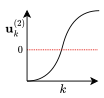
\includegraphics[width=\textwidth]{images/spec_u.svg.pdf}
        % \caption{}
        \label{fig:spec_1}
    \end{subfigure}
    \hfill
    \begin{subfigure}[b]{0.23\textwidth}
        \centering
        \includegraphics[width=\textwidth]{images/spec_g.drawio.svg.pdf}
        % \caption{}
        \label{fig:spec_2}
    \end{subfigure}
    \caption{Plot of the values of $\mathbf{u}^{(2)}$, where each $\mathbf{u}^{(2)}_i$ corresponds to vertex
    $v_i$ in the original sequence, and where $\mathbf{u}^{(2)}_k$ corresponds to $v_k$ in the reordered sequence, such that $\mathbf{u}^{(2)}_1 < \mathbf{u}^{(2)}_2 < \dots < \mathbf{u}^{(2)}_n$ (left).
    The graph partitions corresponding to this ordering (right), with the threshold $\epsilon = 0$ defining the cut (right).
    }
    \label{fig:spec}
\end{figure}
    
    \begin{algorithm}
    \caption{Spectral bisection.}
    \label{alg:spec}
    \begin{algorithmic}[1]
        \Require Graph \( G = (\mathcal{V}, \mathcal{E}) \)
    \Ensure A bisection of \( G \) into \(\mathcal{V}_1\) and \(\mathcal{V}_2\)
    \Function{spectral\_part}{graph $G$}
        \State Form the Laplacian matrix \(\mathbf{L}\)
        \State Compute the 2nd smallest eigenval. \(\lambda^{(2)}\) and eigenvec. \(\mathbf{u}^{(2)}\)
        \State Set 0 or the median of \(\mathbf{u}^{(2)}\) as threshold \(\epsilon\)
        \State Set \(\mathcal{V}_1 := \{v_i \in \mathcal{V} \mid u_i< \epsilon\}\), \(\mathcal{V}_2 := \{v_i \in \mathcal{V} \mid u_i \geq \epsilon\}\)
        \State \Return \(\mathcal{V}_1, \mathcal{V}_2\)
    \EndFunction
    \end{algorithmic}
\end{algorithm}

    % Spectral bisection method implemented in \texttt{GraphLab.jl} can be executed with:

    \begin{lstlisting}[language=Julia]
    GraphLab.part_spectral(A)
    \end{lstlisting}

    Its sole input is the adjacency matrix \texttt{A} and its output a vector assigning each node to partition $1$ or $2$.


%%%%%%%%%%%%%%%%%%%%%%%%%%%%%%%%%%%%%%%%%%%%%%%%%%%%%%%%%%%%%%
% Hybrid bisection
%%%%%%%%%%%%%%%%%%%%%%%%%%%%%%%%%%%%%%%%%%%%%%%%%%%%%%%%%%%%%%
    \subsection{Hybrid partitioning algorithms}
    \label{subsec:hybrid}
    Combining the random sphere bisection and the spectral partitioning described in \ref{sub:rand_sphere} and \ref{sub:spec}, hybrid bisection extends spectral methods with
    a geometric layer to enhance partitioning quality, particularly in graphs with an underlying spatial structure. It begins by computing a spectral embedding of the graph, where each vertex $v_i$ is mapped to a point 
    \begin{equation}
        \mathbf{z}_i = \left( \mathbf{u}_i^{(2)}, \dots, \mathbf{u}_i^{(k+1)}\right) \in \mathbb{R}^k,
    \end{equation}
    using the first $k$ nontrivial eigenvectors of the Laplacian matrix. This embedding encodes the global
    connectivity structure of the graph in a low-dimensional space, where geometric separations of the embedded points with the random sphere method lead to sparse graph cuts. This process performs a geometric search over separators, guided by the spectral structure of the graph. The figure~\Cref{fig:spectral-embedding} illustrates the case with $k=2$, where the embedding uses the first two non-trivial Laplacian eigenvectors.
    % 
    \begin{figure}[t]
    \centering
    \includegraphics[width=1.0\linewidth]{images/airfoil_ev.drawio.png}
    \caption{Spectral embedding and random sphere partitioning: the \texttt{airfoil1}~\cite{10.1145/2049662.2049663} graph is first embedded into a 2-dimensional
    spectral space using the eigenvectors associated with the second and third smallest eigenvalues of the graph Laplacian. A separator (shown in red)
    is then selected using the randomized sphere method and mapped back onto original graph.}
    \label{fig:spectral-embedding}
    \end{figure}
    % 
    The hybrid method leverages the algebraic properties of spectral embeddings and effectiveness of random sphere cuts to generate balanced and spatially localized partitions. It's overall complexity is dominated by the spectral stage, $O(mt_k)$ for sparse graphs, where $t_k$ is the number of Lanczos iterations required to compute $k$ nontrivial eigenvectors.

    Geometric spectral partitioning in \texttt{GraphLab.jl} can be executed with:

    \begin{lstlisting}[language=Julia]
    GraphLab.part_geospectral(A; ev=d)
    \end{lstlisting}

    In addition to the adjacency matrix \texttt{A}, it optionally accepts $\texttt{ev}=d$, i.e., the number of nontrivial Laplacian eigenvectors to use for embedding (default: 2).
    
%%%%%%%%%%%%%%%%%%%%%%%%%%%%%%%%%%%%%%%%%%%%%%%%%%%%%%%%%%%%%%
% Recursive bisection
%%%%%%%%%%%%%%%%%%%%%%%%%%%%%%%%%%%%%%%%%%%%%%%%%%%%%%%%%%%%%%
    \subsection{Recursive bisection and nested dissection}
    Recursive bisection and nested dissection are techniques that rely on recursively splitting a graph into smaller subgraphs. While recursive bisection is primarily used to generate multiple balanced partitions, nested dissection applies a recursive strategy to reduce fill-in during sparse matrix factorization~\cite{George73}. This section outlines both methods and their respective algorithmic formulations.
    \subsubsection{Recursive bisection}
    \label{subsub:rec_bi}
    A straightforward and effective strategy for partitioning a graph into $p = 2^q$ parts,
    where $q$ is a positive integer, is recursive bisection, as presented in \Cref{alg:recursive}.
    This algorithm iteratively applies graph bisection, progressively
    subdividing the graph into smaller subgraphs.
    In \texttt{GraphLab.jl}, recursive bisection can be used with any of the bisection algorithms presented in \Cref{subsec:geo,subsec:non-geo}.
    The algorithm is built around a recursive function, \texttt{Recursion}, which takes as inputs:
    \begin{itemize}
        \item $C'$, the current subgraph to be partitioned,
        \item $p'$, the number of partitions into which $C'$ will be further divided, and
        \item $\mathrm{idx}$, an integer tracking the position of the first part of $C'$ in the final partitioning results.
    \end{itemize}
    
    At each recursive step, the subgraph $C'$ is bisected into two approximately balanced parts. The process continues
    until the desired number of partitions, $p = 2^q$, is obtained.
    The total cost is $O(T_{\text{bisect}}(n, m) \log p)$, where $ T_{\text{bisect}}(n, m)$ is the cost of a single bisection method.
    This recursive strategy results in a structured,
    hierarchical decomposition of the graph, making it particularly well suited for load balancing and for reducing communication overhead in parallel finite element and finite difference implementations~\cite{doi:10.1137/S1064827593255135}.
    
    \begin{algorithm}
    \caption{Recursive bisection.}
    \label{alg:recursive}
    \begin{algorithmic}[1]
        \Require Graph \( G = (\mathcal{V}, \mathcal{E}) \)
    \Ensure A $p$-way partition of \( G \)
    \State \(G_p = \{C_1,\dots, C_p\}\)
    \State \(p = 2^l\)
    \Function{rec\_bisection}{graph $G$, number of parts $p$}
        \Function{recursion}{$C'$, $p'$, $\mathrm{idx}$}
            \If{\(p'\) \text{is even}}
                \State \(p' \leftarrow \frac{p'}{2}\)
                \State \(\left(C'_1, C'_2\right)\leftarrow \)\Call{bisection}{$C'$}
                \State \Call{recursion}{$C'_1$, $p'$, $\mathrm{idx}$}
                \State \Call{recursion}{$C'_2$, $p'$, $\mathrm{idx}+p'$}
            \Else
                \State \(C_{\mathrm{idx}} \leftarrow C'\)
            \EndIf
        \EndFunction
         \State \Call{recursion}{$C$, $p$, $1$}
         \State \Return \(G_p\)
    \EndFunction
    \end{algorithmic}
\end{algorithm}

    \texttt{GraphLab.jl} provides a recursive interface for all partitioning algorithms described in \Cref{sec:algo}, which can be invoked with:

    \begin{lstlisting}[language=Julia]
    GraphLab.recursive_bisection(method, k, 
        A, coords)
    \end{lstlisting}

    Here, \texttt{method} is any partitioning function available in the package, \texttt{k} is the desired number of partitions (automatically rounded up to the nearest power of two if needed), \texttt{A} is the graph's adjacency matrix, and \texttt{coords} is an optional argument (default: \texttt{nothing}) used only for coordinate-based methods. The function returns a vector assigning each node a label from 1 to \texttt{k}, indicating its partition membership.


    \subsubsection{Nested dissection}
    The nested dissection ordering algorithm is a multilevel heuristic designed to minimize fill-in, i.e., the creation of nonzero entries during sparse matrix factorizations~\cite{George73}.
    It recursively partitions a graph $G$ through the identification of balanced vertex separators, which are removed to decompose $G$ into disconnected components. The same procedure is then applied recursively to each subgraph.
    Unlike standard recursive bisection, which directly bisects the graph into two parts, nested dissection introduces an intermediate step: the explicit computation of a node separator whose removal divides the problem into independent subproblems.
    To compute the separator, border vertices are first identified between the two subdomains resulting from the initial bisection. These vertices induce a bipartite graph, in which edges represent adjacency across the partition boundary. A maximum matching is then computed on this bipartite graph and a minimum vertex cover can be derived from it~\cite{bondy1976graph, storer2012introduction}, providing an efficient approximation of a small separator. The selected separator vertices are removed, and the nested dissection proceeds recursively on the resulting components.
    The final ordering $\pi$ places all separator vertices after the recursively ordered interior vertices, yielding a global vertex ordering that reveals a hierarchical block structure in the reordered matrix.
    The complexity of nested dissection is $O(T_{\text{bisect}}(n,m) \log n)$, where $T_{\text{bisect}}(n,m)$ denotes the cost of a single graph bisection.
    The overall process is outlined in \Cref{alg:nested_dis}.

    This strategy is widely used in the symbolic
    factorization phase of sparse direct solvers, where it
    facilitates the construction of efficient elimination
    trees and reduces both fill-in and memory overhead
    during numerical factorization~\cite{Bollhöfer2020}.
    Nested dissection can be implemented using the
    partitioning methods presented in \Cref{subsec:geo}
    and \Cref{subsec:non-geo} for computing the node
    separator. \Cref{fig:nd_perm_results} illustrates how
    different separator methods permute the adjacency
    matrix into a
    hierarchy of interior and separator blocks, yielding
    distinctive banded or clustered nonzero patterns.
    The differences between the separator methods are
    reflected in the number of nonzero entries in the
    Cholesky factor~\cite{George73}.
    
    \begin{figure}[h]
    \centering
    \begin{subfigure}[b]{0.23\textwidth}
        \centering
        \includegraphics[width=\textwidth]{images/nd_3elt_orig.png}
        \caption{\centering Original adjacency, Cholesky $\text{nnz}=93892$.}
        \label{fig:nd_original}
    \end{subfigure}
    \hfill
    \begin{subfigure}[b]{0.23\textwidth}
        \centering
        \includegraphics[width=\textwidth]{images/nd_3elt_coord.png}
        \caption{\centering Coordinate bisection,  Cholesky $\text{nnz}=89566$}
        \label{fig:nd_coord}
    \end{subfigure}

    \vskip\baselineskip  % Adds vertical space between the rows

    \begin{subfigure}[b]{0.23\textwidth}
        \centering
        \includegraphics[width=\textwidth]{images/nd_3elt_inert.png}
        \caption{\centering Inertial bisection,  Cholesky $\text{nnz}=89653$}
        \label{fig:nd_inert}
    \end{subfigure}
    \hfill
    \begin{subfigure}[b]{0.23\textwidth}
        \centering
        \includegraphics[width=\textwidth]{images/nd_3elt_spec.png}
        \caption{\centering Spectral bisection,  Cholesky $\text{nnz}=89110$}
        \label{fig:nd_spec}
    \end{subfigure}

    \caption{Comparison of the (a) original adjacency matrix of the \texttt{3elt} graph against three nested dissection reoderings obtained using (b) coordinate, (c) inertial,  and (d) spectral-based separators. Number of nonzeros (nnz) in the Cholesky factor are reported in the subcaptions.}
    \label{fig:nd_perm_results}
\end{figure}

    


    \begin{algorithm}
    \caption{Nested dissection ordering.}
    \label{alg:nested_dis}
    \begin{algorithmic}[1]
        \Require Adj. matrix \( A \), partitioning \textsc{method}, minimum separator size $\mathrm{minsep}$
        \Ensure Permutation vector \(\pi\) s.t. \(A[\pi, \pi]\) has reduced fill-in
        \Function{nested\_dis}{$A$, \textsc{method}, $\mathrm{coords}$ (opt.), $\mathrm{minsep}$}
            \State Identitfy connected components of \(A\)
            \State Initialize permutation vector \(\pi\)

            \For{each component \(C\)}
                \If{\(|C| \leq \mathrm{minsep}\)}
                    \State Apply minimum degree ordering on \(A[C, C]\)
                \Else
                    \State Bisect \(C \rightarrow C_1, C_2\) via \textsc{method} 
                    \State Identify separator nodes between \(C_1\) and \(C_2\)
                    \State Recursively compute orderings:
                    \State \hspace{2em}$\pi_1 \gets$ \Call{nested\_dis}{$A[C_1, C_1]$}
                    \State \hspace{2em}$\pi_2 \gets$ \Call{nested\_dis}{$A[C_2, C_2]$}
                    \State Combine \(\pi_C \gets [\pi_1, \pi_2, \text{separator}]\)
                \EndIf
                \State Insert \(\pi_C\) into global permutation \(\pi\)
            \EndFor
            
            \State \Return \(\pi\)
        \EndFunction
    \end{algorithmic}
\end{algorithm}

    The nested dissection provided by \texttt{GraphLab.jl} is called using:

    \begin{lstlisting}[language=Julia]
    GraphLab.nested_dissection(A, method; 
        coords, minsep=5)
    \end{lstlisting}

    The inputs are the adjacency matrix \texttt{A}, any partitioning \texttt{method} from \texttt{GraphLab.jl}, and the node coordinates \texttt{coords} if required by the partitioner. An optional argument \texttt{minsep} specifies the minimum separator size (default: 5). The output is a permutation vector representing the nested dissection ordering.
    
% \end{document}

\section{Framework and tools for graph bisection}
    \label{sec:framwork}
    %%%%%%%%%%%%%%%%%%%%%%%%%%%%%%%%%%%%%%%%%%%%%%%%%%%%%%%%%%%%%%
% Framework
%%%%%%%%%%%%%%%%%%%%%%%%%%%%%%%%%%%%%%%%%%%%%%%%%%%%%%%%%%%%%%
\documentclass[../paper.tex]{subfiles}
\begin{document}
    While a variety of algorithms exist for performing graph bisection, as discussed in \Cref{sec:algo},
    an integrated framework is essential to streamline the entire workflow
    --- from graph creation and algorithm execution to benchmarking and visualization.
    Existing tools often address only specific aspects of this process, but lack
    cohesive support for tasks like generating graphs, managing input/output, benchmarking performance, and visually interpreting results.
    % This fragmentation complicates systematic comparisons
    % between different methods.
    We propose a comprehensive framework for graph bisection, designed to unify these components into a single, structured workflow.
    The framework consists of the following core modules:
    \begin{enumerate}
        \item \textbf{Graph creation}: Generating and managing graphs suitable for the application of various partitioning algorithms.
        \item \textbf{Graph bisection}: Implementing the bisection methods detailed in \Cref{sec:algo}.
        \item \textbf{Benchmarking}: Measuring and comparing algorithm performance according to graph-cut criteria.
        \item \textbf{Visualization}: Providing visual representations of graphs and their partitions to facilitate analysis and comparison.
        \item \textbf{Integration}: Enabling interoperability with existing graph partitioning tools and libraries.
    \end{enumerate}
    % By consolidating these elements, \texttt{GraphLab.jl} aims to offer a seamless and reproducible workflow for studying and applying graph bisection techniques.
%%%%%%%%%%%%%%%%%%%%%%%%%%%%%%%%%%%%%%%%%%%%%%%%%%%%%%%%%%%%%%
% Graph creation
%%%%%%%%%%%%%%%%%%%%%%%%%%%%%%%%%%%%%%%%%%%%%%%%%%%%%%%%%%%%%%  
    % \subsection{Graph creation}
    % \label{subsec:graph_creat}
    % The first step in the framework involves preparing the graph for bisection.
    % This process begins with the input of a file containing either the graph's adjacency matrix, vertex coordinates, or both. Supported format includes \texttt{.csv}, which typically stores coordinate data, and \texttt{.mat},
    % which is a MATLAB format commonly used to numerical data storage. The procedure is outlined as follows:
    % \begin{enumerate}
    %     \item \textbf{Input file parsing}: The user provides a filename (e.g., \texttt{airfoil1} or \texttt{mesh3e1}) containing the graph data. If the file is in
    %     \texttt{.csv} format, it is assumed to store a list of vertex coordinates. If the file is in
    %     \texttt{.mat} format, it may contain multiple variables, typically including
    %     the adjacency matrix $\mathbf{A}$ and the coordinates.
    
    %     \item \textbf{File type detection}: The program identifies the file format and 
    %     extracts the relevant information; if an adjacency matrix is present, it is loaded directly; if only the coordinates are provided, further processing is required to construct the adjacency matrix.
    
    %     \item \textbf{Adjacency matrix construction}: If $\mathbf{A}$ is not provided explicitly, it is generated from the vertex coordinates based on spatial proximity or another specified rule, such as $k$-nearest neighbors.
    
    %     \item \textbf{Symmetry check and symmetrization}: Since the framework assumes undirected graphs, the adjacency matrix is checked for symmetry. If $\mathbf{A}$ is not symmetric, it is symmetrized using
    %     \begin{equation}
    %         \mathbf{A}_{\mathrm{sym}} = \frac{\mathbf{A}+\mathbf{A}^T}{2}
    %     \end{equation}
    %     This ensures compatibility with the bisection algorithms presented in \ref{sec:algo}.
    
    %     \item \textbf{Output}: The procedure returns the adjacency matrix $\mathbf{A}$ and a vertex
    %     coordinates (if available). These components serve as inputs for subsequent steps, such
    %     as graph visualization and partitioning.
    % \end{enumerate}
    % This process leverages the functionalities of the \texttt{DelimitedFiles.jl}\footnote{\url{https://docs.julialang.org/en/v1/stdlib/DelimitedFiles/}} and \texttt{MAT.jl}\footnote{\url{https://github.com/JuliaIO/MAT.jl}} packages to handle file parsing and data extraction.

    \subsection{Graph creation}
    \label{subsec:graph_creat}
    
    Graphs used in the framework can either be syntheticaly generated or loaded from external files.
    Synthetic graphs are typically generated as $n \times m$ grids with a rotation of $\theta$ radians.
    % using functions like \texttt{GraphLab.grid\_graph(\(n\), \(m\), \(\theta\))}, which creates a $n \times m$ grid rotated by \(\theta\) radians.
    Alternatively, users can upload a \texttt{mat} file with an adjacency matrix and optional coordinate, or a \texttt{csv} file with coordinates only, from which the adjacency matrix is constructed using $k$-nearest neighbors.
    % Alternatively, users may upload a \texttt{.mat} or \texttt{.csv} file. If a \texttt{.mat} file is provided, it is expected to contain an adjacency matrix \(\mathbf{A}\) and, optionally, vertex coordinates. A \texttt{.csv} file is assumed to provide only the coordinates, in which case the adjacency matrix can be built using $k$-nearest neighbors.
    % In all cases, the graph is assumed to be undirected; if \(\mathbf{A}\) is not symmetric, it can be symmetrized:
    % \begin{equation}
    %     \mathbf{A}_{\mathrm{sym}} = \frac{\mathbf{A} + \mathbf{A}^\top}{2}
    % \end{equation}
    The file parsing and data loading are handled by the external packages \texttt{MAT.jl}\footnote{\url{https://github.com/JuliaIO/MAT.jl}} and \texttt{DelimitedFiles.jl}\footnote{\url{https://docs.julialang.org/en/v1/stdlib/DelimitedFiles/}}.
    
    % This preprocessing yields the adjacency matrix and coordinates needed for subsequent partitioning and visualization steps. File parsing and data loading rely on \texttt{MAT.jl}\footnote{\url{https://github.com/JuliaIO/MAT.jl}} and \texttt{DelimitedFiles.jl}\footnote{\url{https://docs.julialang.org/en/v1/stdlib/DelimitedFiles/}}.

%%%%%%%%%%%%%%%%%%%%%%%%%%%%%%%%%%%%%%%%%%%%%%%%%%%%%%%%%%%%%%
% Benchmarking
%%%%%%%%%%%%%%%%%%%%%%%%%%%%%%%%%%%%%%%%%%%%%%%%%%%%%%%%%%%%%%
    % \subsection{Benchmarking}
    % \label{subsec:bench}
    % The framework includes two benchmarking procedures to evaluate the performance of the implemented bisection methods, focusing on both edge cut and partition balance ratio as key evaluation metrics. Additional metrics can be
    % incorporated in future analyses to provide a more comprehensive assessment.
    % \begin{enumerate}
    %     \item \textbf{Bisection method comparison}: This benchmark compares different bisection methods across various input meshes. The partitioning quality is assessed using both edge cut and partition balance ratio as performance metrics.
    %     \item \textbf{Recursive bisection comparison}: This benchmark assesses recursive bisection strategies applied to different meshes and partitioning methods. The graph is partitioning into $p=8$ and
    %     $p=16$ subdomains, and both edge cut and balance ratio are measured to assess the efficiency of the recursive process. 
    % \end{enumerate}
    
    % The results are presented in tables generated using \texttt{PrettyTables.jl}\footnote{\url{https://ronisbr.github.io/PrettyTables.jl/stable/}} for structured and clear visualization. While
    % edge cut and balance ratio serve as primary evaluation criteria, the framework is designed to accommodate additional metrics in future extensions, such as partition balance and computational efficiency.

    \subsection{Benchmarking}
    \label{subsec:bench}
    
    The framework includes two example scripts, provided in the \texttt{examples} directory of the \texttt{GraphLab.jl} package, to benchmark the implemented graph bisection strategies. The edge cut is defined as the number of edges crossing between partitions, while the balance ratio measures how evenly the graph is divided.
    
    \begin{enumerate}
        \item \texttt{ex1.jl}: Benchmarks multiple bisection methods across a set of mesh inputs. For each method and mesh, it evaluates the edge cut and partition balance. Since all resulting balance ratios are very close to one, we report the achieve edge cut values in \Cref{tab:edgecut-table}.
    
        \item \texttt{ex2.jl}: Benchmarks recursive bisection. The graph is recursively partitioned into $p = 8$ and $p = 16$ subdomains using a given base bisection method. Edge cut and balance are recorded for each case.
        % Edge cut values are reported in Table~\ref{tab:swiss-combined}.
    \end{enumerate}

    \begin{table*}[t]
        \tbl{Edge cuts for each method and mesh.}{
        \begin{tabular}{|l|c|c|c|c|c|c|c|}
        \hline
        \textbf{Mesh} & coordinate & inertial & randsphere & adaptive sfc & spectral & geospectral & METIS \\
        % \hline
        \texttt{3elt}             & 172 & 209 & 94 & 224 & 117 & 117 & 90 \\
        \texttt{airfoil1}         & 94 & 94 & 93 & 98 & 132 & 132 & 73 \\
        \texttt{barth4}           & 206 & 194 & 130 & 208 & 127 & 127 & 100 \\
        \texttt{crack}            & 323 & 377 & 275 & 353 & 233 & 233 & 200 \\
        \texttt{mesh1e1}          & 18 & 19 & 18 & 18 & 18 & 18 & 17 \\
        \texttt{mesh2e1}          & 37 & 47 & 36 & 40 & 35 & 35 & 34 \\
        \texttt{mesh3e1}          & 17 & 32 & 18 & 21 & 30 & 20 & 18 \\
        \texttt{mesh3em5}         & 17 & 32 & 18 & 21 & 18 & 20 & 18 \\
        \texttt{netz4504\_dual}   & 25 & 30 & 23 & 25 & 23 & 23 & 20 \\
        \texttt{stufe}            & 16 & 16 & 16 & 16 & 16 & 16 & 17 \\
        \texttt{ukerbe1}          & 27 & 28 & 34 & 34 & 28 & 28 & 30 \\
        \hline
        \end{tabular}}
        \label{tab:edgecut-table}
    \end{table*}

    % \begin{table}[h]
    %     \tbl{Edge cut values for recursive bisection into 8 and 16 subdomains on \texttt{Swiss\_graph}.}{
    %     \begin{tabular}{|l|c|c|}
    %     \hline
    %     \textbf{Method} & \textbf{8-way} & \textbf{16-way} \\
    %     \hline
    %     Recursive:\texttt{coordinate} & 520 & 858 \\
    %     Recursive:\texttt{inertial}   & 500 & 828 \\
    %     Recursive:\texttt{spectral}   & 459 & 753 \\
    %     \texttt{METIS\_rec}           & 389 & 699 \\
    %     \texttt{METIS\_kway}          & 392 & 693 \\
    %     \hline
    %     \end{tabular}}
    %     \label{tab:swiss-combined}
    % \end{table}
        
    % All results are saved and exported using \texttt{CSV.jl}. While edge cut and balance are the primary metrics, the framework can be extended to track additional criteria such as separator size or runtime.
    
%%%%%%%%%%%%%%%%%%%%%%%%%%%%%%%%%%%%%%%%%%%%%%%%%%%%%%%%%%%%%%
% Visualization
%%%%%%%%%%%%%%%%%%%%%%%%%%%%%%%%%%%%%%%%%%%%%%%%%%%%%%%%%%%%%%
    \subsection{Visualization}
    \label{subsec:visu}
    To generate visual representations of graph partitions, this steps requires the adjacency matrix $\mathbf{A}$, the vertex coordinates, and the corresponding partition information. The framework integrates multiple Julia packages to ensure clear visualization:
    \begin{itemize}
        \item \textbf{\texttt{SGtSNEpi.jl}}\footnote{\url{https://github.com/fcdimitr/SGtSNEpi.jl}}: A scalable tools for embedding and plotting large graphs, addressing challenges posed by visualization libraries that struggle with size constraints.
        \item \textbf{\texttt{Graphs.jl}}\footnote{\url{https://juliagraphs.org/Graphs.jl/}}: Provides essential graph operations and data structures.
        \item \textbf{\texttt{CairoMakie.jl}}\footnote{\url{https://docs.makie.org/stable/explanations/backends/cairomakie.html}}: Enables the creation customizable plots suitable for publication.
        \item \textbf{\texttt{Colors.jl}}\footnote{\url{https://juliagraphics.github.io/Colors.jl/}}: Manages color palettes for visually distinguishing partitions.
    \end{itemize}

    Visualizations of the results produced by the scripts introduced in \Cref{subsec:bench} are presented in \Cref{fig:ex1_results} and \Cref{fig:ex2_results}.

    \begin{figure}[h]
    \centering
    \begin{subfigure}[b]{0.23\textwidth}
        \centering
        \includegraphics[width=\textwidth,  trim={100pt 74pt 0 0}, clip]{images/ex1_airfoil1_coordinate.png}
        \caption{Coordinate bisection}
        \label{fig:ex1_coord}
    \end{subfigure}
    \hfill
    \begin{subfigure}[b]{0.23\textwidth}
        \centering
        \includegraphics[width=\textwidth,  trim={100pt 74pt 0 0}, clip]{images/ex1_airfoil1_inertial.png}
        \caption{Inertial bisection}
        \label{fig:ex1_inertial}
    \end{subfigure}

    \vskip\baselineskip  % Adds vertical space between the rows

    \begin{subfigure}[b]{0.23\textwidth}
        \centering
        \includegraphics[width=\textwidth,  trim={100pt 74pt 0 0}, clip]{images/ex1_airfoil1_spectral.png}
        \caption{Spectral bisection}
        \label{fig:ex1_spectral}
    \end{subfigure}
    \hfill
    \begin{subfigure}[b]{0.23\textwidth}
        \centering
        \includegraphics[width=\textwidth,  trim={100pt 74pt 0 0}, clip]{images/ex1_airfoil1_metis.png}
        \caption{Bisection using \texttt{METIS}}
        \label{fig:ex1_metis}
    \end{subfigure}

    \caption{Visualization of four graph bisection methods applied to the \texttt{airfoil1} mesh (4253 nodes and 12289 edges), illustrating differences in partitioning structure and edge cuts.}
    \label{fig:ex1_results}
\end{figure}


    \begin{figure}[h]
    \centering
    \begin{subfigure}[b]{0.23\textwidth}
        \centering
        \includegraphics[width=\textwidth,  trim={98pt 70pt 0 0}, clip]{images/ex2_Swiss_graph_coordinate.png}
        \caption{\centering Recursive coordinate bisection, RCut~=~6.15}
        \label{fig:ex2_coord}
    \end{subfigure}
    \hfill
    \begin{subfigure}[b]{0.23\textwidth}
        \centering
        \includegraphics[width=\textwidth,  trim={98pt 70pt 0 0}, clip]{images/ex2_Swiss_graph_inertial.png}
        \caption{\centering Recursive inertial bisection, RCut~=~5.93}
        \label{fig:ex2_inertial}
    \end{subfigure}

    \vskip\baselineskip  % Adds vertical space between the rows

    \begin{subfigure}[b]{0.23\textwidth}
        \centering
        \includegraphics[width=\textwidth,  trim={98pt 70pt 0 0}, clip]{images/ex2_Swiss_graph_spectral.png}
        \caption{\centering Recursive spectral bisection, RCut~=~5.39}
        \label{fig:ex2_spectral}
    \end{subfigure}
    \hfill
    \begin{subfigure}[b]{0.23\textwidth}
        \centering
        \includegraphics[width=\textwidth,  trim={98pt 70pt 0 0}, clip]{images/ex2_Swiss_graph_metis_rec.png}
        \caption{\centering Recursive \texttt{METIS} bisection, RCut~=~5.01}
        \label{fig:ex2_metis}
    \end{subfigure}

    \caption{Comparison of four graph recursive bisection methods applied to the \texttt{Swiss\_graph}\protect\footnotemark{} (4468 nodes and 15230 edges), illustrating differences in the 16-way recursive partitioning and the associated ratio cut.}
    \label{fig:ex2_results}
\end{figure}
\footnotetext{\url{https://github.com/lechekhabm/GraphLab.jl/tree/main/examples/meshes}}


% \begin{figure}
%     \centering

%     \begin{subfigure}[b]{0.45\textwidth}
%         \centering
%         \includegraphics[width=\textwidth, trim={98pt 70pt 0 0}, clip]{images/ex2_Swiss_graph_coordinate.png}
%         \caption{Recursive coordinate bisection}
%         \label{fig:ex2_coord}
%     \end{subfigure}

%     \vskip\baselineskip

%     \begin{subfigure}[b]{0.45\textwidth}
%         \centering
%         \includegraphics[width=\textwidth, trim={98pt 70pt 0 0}, clip]{images/ex2_Swiss_graph_inertial.png}
%         \caption{Recursive inertial bisection}
%         \label{fig:ex2_inertial}
%     \end{subfigure}

%     \vskip\baselineskip

%     \begin{subfigure}[b]{0.45\textwidth}
%         \centering
%         \includegraphics[width=\textwidth, trim={98pt 70pt 0 0}, clip]{images/ex2_Swiss_graph_spectral.png}
%         \caption{Recursive spectral bisection}
%         \label{fig:ex2_spectral}
%     \end{subfigure}

%     \vskip\baselineskip

%     \begin{subfigure}[b]{0.45\textwidth}
%         \centering
%         \includegraphics[width=\textwidth, trim={98pt 70pt 0 0}, clip]{images/ex2_Swiss_graph_metis_rec.png}
%         \caption{Recursive spectral bisection}
%         \label{fig:ex2_metis}
%     \end{subfigure}

%     \caption{Recursive bisection of the \texttt{Swiss\_graph} mesh using different methods. Each partition result shows the division into $p = 16$ subdomains.}
%     \label{fig:ex2_results}
% \end{figure}
   %  \begin{figure}[h!]
    \centering
    \begin{subfigure}[b]{0.23\textwidth}
        \centering
        \includegraphics[trim={0 0 0 2.5cm}, clip, width=1.1\textwidth]{images/plot_ex_1.png}
        % \caption{}
        \label{fig:visu_simple}
    \end{subfigure}
    \hfill
    \begin{subfigure}[b]{0.23\textwidth}
        \centering
        \includegraphics[trim={0 0 0 2.5cm}, clip, width=1.1\textwidth]{images/plot_ex_2.png}
        % \caption{}
        \label{fig:visu_2part}
    \end{subfigure}
    \caption{Graph visualization example and the corresponding result after applying
    a bisection. The original graph structure is shown on the left, while the right 
    visualization highlights the two obtained partitions.}
    \label{fig:visu}
\end{figure}
%%%%%%%%%%%%%%%%%%%%%%%%%%%%%%%%%%%%%%%%%%%%%%%%%%%%%%%%%%%%%%
% Integration
%%%%%%%%%%%%%%%%%%%%%%%%%%%%%%%%%%%%%%%%%%%%%%%%%%%%%%%%%%%%%%
    % \subsection{Integration with external graph partitioning software}
    % \label{subsec:integr}
    % The framework supports interoperability with widely used graph partitioning tools, allowing
    % users to incorporate advanced algorithms alongside the provided methods.
    % We provide guidelines and examples demonstrating how to integrate external software into
    % \texttt{GraphLab.jl}.
    % The proposed integration workflow follows these steps:

    %     \begin{enumerate}
    %         \item \textbf{Graph file generation}: Convert the symmetric adjacency matrix into a format compatible with external tools. The standard format includes:
    %             \begin{itemize}
    %                 \item The first line specifying the number of nodes and edges.
    %                 \item Each subsequent line representing a node, listing its neighbors as space-separated integers.
    %             \end{itemize}
                
    %         \item \textbf{Executable path retrieval and validation}: Retrieve the path of the external partitioning software from environment variables and ensure its existence.
            
    %         \item \textbf{Error handling}: Verify the exit code to detect execution failures or misconfigurations.
            
    %         \item \textbf{Partition file retrieval}: Load the partition file generated by the external software.
            
    %         \item \textbf{Partition assignment}: Parse the output and return the partitions as a vector for further processing within the framework.
    %     \end{enumerate}

    % Notable partitioning software that can be integrated include:

    %     \begin{itemize}
    %         \item \textbf{METIS}: A widely used and robust multilevel recursive partitioning strategy for large graphs and meshes\cite{4302760}. It can be accessed through the \texttt{METIS.jl} package\footnote{\url{https://github.com/KarypisLab/METIS}}, which provides a Julia interface to METIS functionalities.

    %         \item \textbf{KaHIP}: A state-of-the-art graph partitioning framework\footnote{\url{https://github.com/KaHIP/KaHIP}} that employs combinatorial optimizations and iterative refinement techniques to produce high-quality, balanced partitions\cite{DBLP:conf/wea/SandersS13}.

    %         \item \textbf{MDC}: An experimental multilevel diffusion clustering techniques based on \texttt{Graclus}\cite{10.1145/1081870.1081948, 4302760}. It leverages diffusion principles to enhance partitioning flexibility through a tunable diffusion parameter\cite{Lechekhab2024MDC}.
    %     \end{itemize}

    % By providing structured workflows and documentation on integrating these tools, we aim to enable users to leverage diverse partitioning methods within a unified research and experimentation environment. Examples demonstrating practical implementations of these integration are available in the documentation of \texttt{GraphLab.jl}.

    
    % To provide flexibility and access well-established graph partitioning techniques, our framework includes interfaces to several partitining algorithms. These include \texttt{METIS} (via \texttt{METIS.jl}), \texttt{KaHIP}, \texttt{Graclus}, and \texttt{Multilevel Diffusion Clustering} (MDC) implemented in \texttt{C}. Each of these algorithms follows distinct principles and trade-offs, making them suitable of different graph partitiong tasks. The integration is designed to allow users to seamlessly call these external methods from Julia, either through direct packages interfaces or system-level calls.
    
    % \subsubsection{METIS --- Multilevel Recursive Graph Partitioning}
    % \texttt{METIS}\footnote{\url{https://github.com/KarypisLab/METIS}} is a widely used and robust graph partitioning library designed for
    % large-scale applications. It employs a multilevel recursive partitioning strategy that balances
    % computational efficiency and partition quality\cite{4302760}. The algorithm has been extensively used in
    % domains such as scientific computing, high-performance computing, and network analysis.
    % Our framework uses the \texttt{METIS.jl}\footnote{\url{https://github.com/JuliaSparse/Metis.jl}} package, a Julia wrapper around the \texttt{METIS} library that offers direct execution of partitioning routines.
    
    % \subsubsection{KaHIP --- Karlsruhe High-Quality Patritioning}
    % \texttt{KaHIP}\footnote{\url{https://github.com/KaHIP/KaHIP}} is a state-of-the-art graph partitioning framework designed to produce high-quality balanced partitions while minimizing edge cut\cite{DBLP:conf/wea/SandersS13}. Unlike traditional partitioning methods that prioritize speed, \texttt{KaHIP} emphasizes partition quality by integrating combinatorial optimizations and iterative refinement techniques. \texttt{KaHIP} is integrated into our framework via a Julia Bash interface, where the partitioning process is executed as an external call.
    
    % \subsubsection{Graclus --- Spectral and Multilevel Clustering}
    % \texttt{Graclus}\footnote{\url{https://www.cs.utexas.edu/~dml/Software/graclus.html}} is a graph clustering algorithm designed to minimized normalized cut and ratio cut objectives efficiently. It leverages the mathematical equivalence between general cut or association objectives and the weighted kernel $k$-means objective\cite{10.1145/1081870.1081948, 4302760}. By integrating \texttt{Graclus} into our framework, we provide users with a Julia interface allowing for seamless interaction with \texttt{Graclus} while maintaining a consistent workflow for benchmarking and visualization.
    
    % \subsubsection{MDC --- Multilevel Diffusion Clustering}
    % The \texttt{MDC}\footnote{\url{https://github.com/lechekhabm/MDC}\add{! repo needs to be cleaned or removed from the paper}} algorithm leverages diffusion principles to minimize the normalized cut, adds flexibility through a diffusion parameter, and retrieves high-quality partitions in a multilevel fashion without computing eigenpairs\cite{Lechekhab2024MDC}. Comparison with modern multilevel multilevel graph clustering packages reveal that this method can improve the clustering of graphs both in terms of balanced cut criteria and classification accuracy.
\end{document}

\section{Installation and demonstration}
    \label{sec:demo}
    %%%%%%%%%%%%%%%%%%%%%%%%%%%%%%%%%%%%%%%%%%%%%%%%%%%%%%%%%%%%%%
% Installation and demonstration
%%%%%%%%%%%%%%%%%%%%%%%%%%%%%%%%%%%%%%%%%%%%%%%%%%%%%%%%%%%%%%
% \documentclass[../paper.tex]{subfiles}
% \begin{document}
    To install the package from GitHub\footnote{\url{https://github.com/lechekhabm/GraphLab.jl}} and integrate it into the working environment, the following steps are required:

    \begin{enumerate}
        \item Add \texttt{GraphLab.jl} to the project using the Julia command:
\begin{lstlisting}[language = Julia]
using Pkg
Pkg.add(url="https://github.com/lechekhabm/GraphLab.jl")
\end{lstlisting}
        \item As a basic example for graph partitioning, the adjacency matrix $\mathbf{A}$ and vertex coordinates
        are first constructed from the input data.
        Here, we generate a synthetic $10 \times 50$ rectangular grid graph rotated by an angle of $\pi/3$ radians.
        Spectral bisection is then applied to compute the partition $p$, followed by visualizing and exporting the figure of the partitioned graph. The process is executed with the following commands:
        \newline
\begin{lstlisting}[language = Julia]
using GraphLab
A, coords = GraphLab.grid_graph(10, 50, π/3)
p = GraphLab.part_spectral(A)
GraphLab.draw_graph(A, coords, p, file_name="test.png")
\end{lstlisting}

        % The package automatically installs the following dependencies: \texttt{Arpack}, \texttt{CairoMakie}, \texttt{Colors}, \texttt{Graphs}, \texttt{LinearAlgebra}, \texttt{Metis}, \texttt{SparseArrays}, \texttt{Statistics}, \texttt{AMD}, \texttt{GraphsMatching}, \texttt{JuMP}, and \texttt{Cbc}.
        % For extended functionality, additional packages such as \texttt{DelimitedFiles}, \texttt{MAT}, \texttt{Plots}, and \texttt{PrettyTables} may be required.
    \end{enumerate}
Further details about the package and its functionalities can be found in the online documentation\footnote{\url{https://lechekhabm.github.io/GraphLab.jl/dev/}}.
    
%%%%%%%%%%%%%%%%%%%%%%%%%%%%%%%%%%%%%%%%%%%%%%%%%%%%%%%%%%%%%%
% Demonstration
%%%%%%%%%%%%%%%%%%%%%%%%%%%%%%%%%%%%%%%%%%%%%%%%%%%%%%%%%%%%%%
    % \subsection{Demonstration}
    % The package includes two example scripts that illustrate the usage of the framework for benchmarking and comparing various graph partitioning methods. These scripts are available in the `examples/` directory within the package and can be executed directly.



%%%%%%%%%%%%%%%%%%%%%%%%%%%%%%%%%%%%%%%%%%%%%%%%%%%%%%%%%%%%%%
% PLOT TEST
%%%%%%%%%%%%%%%%%%%%%%%%%%%%%%%%%%%%%%%%%%%%%%%%%%%%%%%%%%%%%%



%%%%%%%%%%%%%%%%%%%%%%%%%%%%%%%%%%%%%%%%%%%%%%%%%%%%%%%%%%%%%%
% Ex 1
%%%%%%%%%%%%%%%%%%%%%%%%%%%%%%%%%%%%%%%%%%%%%%%%%%%%%%%%%%%%%%
    % \subsubsection{Example 1: Comparing partitioning methods}
    % This example compares various graph partitioning methods, including coordinate bisection, inertial bisection, spectral bisection and bisection using \texttt{METIS}. The script \texttt{ex1.jl} evaluates these methods across a series of different graphs, providing insights into their performance and effectiveness, as illustrated in \Cref{fig:ex1_results}. 
    % \begin{figure}[h]
    \centering
    \begin{subfigure}[b]{0.23\textwidth}
        \centering
        \includegraphics[width=\textwidth,  trim={100pt 74pt 0 0}, clip]{images/ex1_airfoil1_coordinate.png}
        \caption{Coordinate bisection}
        \label{fig:ex1_coord}
    \end{subfigure}
    \hfill
    \begin{subfigure}[b]{0.23\textwidth}
        \centering
        \includegraphics[width=\textwidth,  trim={100pt 74pt 0 0}, clip]{images/ex1_airfoil1_inertial.png}
        \caption{Inertial bisection}
        \label{fig:ex1_inertial}
    \end{subfigure}

    \vskip\baselineskip  % Adds vertical space between the rows

    \begin{subfigure}[b]{0.23\textwidth}
        \centering
        \includegraphics[width=\textwidth,  trim={100pt 74pt 0 0}, clip]{images/ex1_airfoil1_spectral.png}
        \caption{Spectral bisection}
        \label{fig:ex1_spectral}
    \end{subfigure}
    \hfill
    \begin{subfigure}[b]{0.23\textwidth}
        \centering
        \includegraphics[width=\textwidth,  trim={100pt 74pt 0 0}, clip]{images/ex1_airfoil1_metis.png}
        \caption{Bisection using \texttt{METIS}}
        \label{fig:ex1_metis}
    \end{subfigure}

    \caption{Visualization of four graph bisection methods applied to the \texttt{airfoil1} mesh (4253 nodes and 12289 edges), illustrating differences in partitioning structure and edge cuts.}
    \label{fig:ex1_results}
\end{figure}

%%%%%%%%%%%%%%%%%%%%%%%%%%%%%%%%%%%%%%%%%%%%%%%%%%%%%%%%%%%%%%
% Ex 2
%%%%%%%%%%%%%%%%%%%%%%%%%%%%%%%%%%%%%%%%%%%%%%%%%%%%%%%%%%%%%%
    % \subsubsection{Example 2: Comparing recursive bisection}
    % This example illustrates recursive bisection using multiple methods, including coordinate bisection, inertial bisection, spectral bisection, and recursive bisection via \texttt{METIS} K-way partitioning. The script \texttt{ex2.jl} generates the results presented in \Cref{fig:ex2_results}
    % \begin{figure}[h]
    \centering
    \begin{subfigure}[b]{0.23\textwidth}
        \centering
        \includegraphics[width=\textwidth,  trim={98pt 70pt 0 0}, clip]{images/ex2_Swiss_graph_coordinate.png}
        \caption{\centering Recursive coordinate bisection, RCut~=~6.15}
        \label{fig:ex2_coord}
    \end{subfigure}
    \hfill
    \begin{subfigure}[b]{0.23\textwidth}
        \centering
        \includegraphics[width=\textwidth,  trim={98pt 70pt 0 0}, clip]{images/ex2_Swiss_graph_inertial.png}
        \caption{\centering Recursive inertial bisection, RCut~=~5.93}
        \label{fig:ex2_inertial}
    \end{subfigure}

    \vskip\baselineskip  % Adds vertical space between the rows

    \begin{subfigure}[b]{0.23\textwidth}
        \centering
        \includegraphics[width=\textwidth,  trim={98pt 70pt 0 0}, clip]{images/ex2_Swiss_graph_spectral.png}
        \caption{\centering Recursive spectral bisection, RCut~=~5.39}
        \label{fig:ex2_spectral}
    \end{subfigure}
    \hfill
    \begin{subfigure}[b]{0.23\textwidth}
        \centering
        \includegraphics[width=\textwidth,  trim={98pt 70pt 0 0}, clip]{images/ex2_Swiss_graph_metis_rec.png}
        \caption{\centering Recursive \texttt{METIS} bisection, RCut~=~5.01}
        \label{fig:ex2_metis}
    \end{subfigure}

    \caption{Comparison of four graph recursive bisection methods applied to the \texttt{Swiss\_graph}\protect\footnotemark{} (4468 nodes and 15230 edges), illustrating differences in the 16-way recursive partitioning and the associated ratio cut.}
    \label{fig:ex2_results}
\end{figure}
\footnotetext{\url{https://github.com/lechekhabm/GraphLab.jl/tree/main/examples/meshes}}


% \begin{figure}
%     \centering

%     \begin{subfigure}[b]{0.45\textwidth}
%         \centering
%         \includegraphics[width=\textwidth, trim={98pt 70pt 0 0}, clip]{images/ex2_Swiss_graph_coordinate.png}
%         \caption{Recursive coordinate bisection}
%         \label{fig:ex2_coord}
%     \end{subfigure}

%     \vskip\baselineskip

%     \begin{subfigure}[b]{0.45\textwidth}
%         \centering
%         \includegraphics[width=\textwidth, trim={98pt 70pt 0 0}, clip]{images/ex2_Swiss_graph_inertial.png}
%         \caption{Recursive inertial bisection}
%         \label{fig:ex2_inertial}
%     \end{subfigure}

%     \vskip\baselineskip

%     \begin{subfigure}[b]{0.45\textwidth}
%         \centering
%         \includegraphics[width=\textwidth, trim={98pt 70pt 0 0}, clip]{images/ex2_Swiss_graph_spectral.png}
%         \caption{Recursive spectral bisection}
%         \label{fig:ex2_spectral}
%     \end{subfigure}

%     \vskip\baselineskip

%     \begin{subfigure}[b]{0.45\textwidth}
%         \centering
%         \includegraphics[width=\textwidth, trim={98pt 70pt 0 0}, clip]{images/ex2_Swiss_graph_metis_rec.png}
%         \caption{Recursive spectral bisection}
%         \label{fig:ex2_metis}
%     \end{subfigure}

%     \caption{Recursive bisection of the \texttt{Swiss\_graph} mesh using different methods. Each partition result shows the division into $p = 16$ subdomains.}
%     \label{fig:ex2_results}
% \end{figure}

%%%%%%%%%%%%%%%%%%%%%%%%%%%%%%%%%%%%%%%%%%%%%%%%%%%%%%%%%%%%%%
% Usage in teaching scenarios
%%%%%%%%%%%%%%%%%%%%%%%%%%%%%%%%%%%%%%%%%%%%%%%%%%%%%%%%%%%%%%
    % \subsection{Usage in teaching scenarios}
    % \texttt{GraphLab.jl} is designed to support educational use, particularly in courses covering graph algorithms, high-performance computing, and scientific computing.
    % By offering an interactive and reproducible environment, the package enables students to experiment with various partitioning techniques, assess their performance, and gain intuition about graph bisection methods.

    % A typical teaching application could involve \texttt{Pluto.jl} or Google Colab notebooks for visualizing and comparing partitioning methods.
    % For instance, an instructor can guide students through partitioning sample meshes, examining the effects of different algorithms on edge cut and balance ratio.
% \end{document}




\section{Conclusion and future works}
    \label{sec:conclusion}
    %%%%%%%%%%%%%%%%%%%%%%%%%%%%%%%%%%%%%%%%%%%%%%%%%%%%%%%%%%%%%%
% Conclusion
%%%%%%%%%%%%%%%%%%%%%%%%%%%%%%%%%%%%%%%%%%%%%%%%%%%%%%%%%%%%%%
% \documentclass[../paper.tex]{subfiles}
% \begin{document}
    In this work, we have presented \texttt{GraphLab.jl}, a
    framework for graph partitioning
    designed to support research and education in graph theory
    and partitioning problems.
    It incorporates fundamental partitioning methods, such as
    coordinate, inertial, and spectral bisection, as well as
    random spheres, space-filling curves, and nested
    dissection.  It additionally offers utilities for
    visualization, benchmarking, and partition quality
    assessment, in an effort to provide a unified environment for
    analyzing and comparing graph partitioning algorithms.
    Ongoing developments aim to broaden the framework's
    capabilities with implementations of additional
    partitioning techniques, of multilevel
    methods~\cite{10938528, DBLP:conf/wea/SandersS13}, and by
    enabling parallel execution~\cite{7859409}, particularly in
    the recursive implementation of geometric-based algorithms.
% \end{document}

    % A key strength of \texttt{GraphLab.jl} lies in its modular design and extensibility.
    % Users can experiment
    % with a diverse range of partitioning algorithms, leveraging both native implementations and external software.
    % The possibility to integrate with \texttt{Pluto.jl} or other notebook interfaces further enhances interactivity, making the framework especially well suited for teaching and exploratory research.
    
    % Ongoing developments aim to broaden the framework's capabilities.
    % Planned features include additional evaluation metrics, such as modularity, to provide more comprehensive assessments of partition quality.
    % Support for further partitioning techniques, particularly label propagation-based methods, is also under active development, alongside performance optimizations to better support large-scale graphs.
\FloatBarrier
\section{Acknowledgment}
The authors gratefully acknowledge the scientific support and HPC resources provided by the Erlangen National High Performance Computing Center (NHR@FAU) of the Friedrich-Alexander-Universität Erlangen-Nürnberg (FAU) under the NHR project j101df. NHR funding is provided by federal and Bavarian state authorities. NHR@FAU hardware is partially funded by the German Research Foundation (DFG) – 440719683
We also would like to acknowledge the financial support of the joint DFG (ID 470857344) and
SNSF (ID 200021L\_204817) project entitled \textit{Numerical Algorithms, Frameworks, and Scalable Technologies for Extreme-Scale Computing}, and the computing  support by a grant from the Swiss National Supercomputing Centre (CSCS)
under project ID u3-31045.

% \bibliographystyle{unsrt}
\input{bib.tex}

\end{document}

% Inspired by the International Journal of Computer Applications template
